\documentclass{report}

%%%%%%%%%%%%%%%%%%%%%%%%%% Загальна інформація %%%%%%%%%%%%%%%%%%%%%%%%%%
\Subject {Системи штучного інтелекту}
\LabTitle{Логістична регресія}
\LabReport{Практична робота \#3}


%----------------------------------------------------
%	  Персональна інформація виконавця завдання
%----------------------------------------------------
\Done{Виконав:}  % Поставте правильне закінчення


\Surname{Стародубець}  % Вкажіть своє прізвище
\Name{Ілля}			% та ім'я
\Group {ІМ-32мп}     % група в якій навчаєтесь
\YearOfStudying {1} % курс навчання


%%%%%%%%%%%%%%%%%%%%%%%%%%	 ПОЧАТОК ЗВІТУ	 %%%%%%%%%%%%%%%%%%%%%%%%
\startDocument


\section{Логістична регресія}

\subsection{Реалізація логістичної регресії}

\subsubsection{Ініціалізувати ваги та зсув}

\begin{lstlisting}[language=Python, style=mypython]
def parameters_inititalization(m):
  # BEGIN_YOUR_CODE
  W = np.random.randn(1, m)
  b = 0.0

  return W, b
  # END_YOUR_CODE
\end{lstlisting}

\subsubsection{Обчислити лінійну комбінацію вхідних ознак та ваг, включачи зсувю Застосувати нелінійну функцію активації (сигмоїду) до отриманого значення з крок 1}

\begin{lstlisting}[language=Python, style=mypython]
# TODO
def forwardPropagate(X, W, b):
  # BEGIN_YOUR_CODE
  z = np.dot(W, X.T) + b
  y_hat = sigmoid(z)

  return z, y_hat
  # END_YOUR_CODE
\end{lstlisting}

\subsubsection{Обчислити усереднену втрату на всьому навчальному наборі даних}

\begin{lstlisting}[language=Python, style=mypython]
# TODO
def cost(n, y_hat, y_true):
  ep = 10E-10
  # BEGIN_YOUR_CODE
  J = -(1 / n) * np.sum(y_true * np.log(y_hat + ep) + (1 - y_true) * np.log(1 -   y_hat + ep))

  return J
  # END_YOUR_CODE 
\end{lstlisting}

\subsubsection{Розрахувати градієнти цільвої функції відносно ваг та зсуву}

\begin{lstlisting}[language=Python, style=mypython]
# TODO
def backwardPropagate(n, X, y_hat, y_true):
  # BEGIN_YOUR_CODE
  dW = (1 / n) * np.dot(y_hat - y_true, X)
  db = (1 / n) * np.sum(y_hat - y_true)

  return dW, db
  # END_YOUR_CODE
\end{lstlisting}

\subsubsection{Оновити ваги та зсув}

\begin{lstlisting}[language=Python, style=mypython]
# TODO
def update(lr, dW, db, W, b):
  # BEGIN_YOUR_CODE
  W -= lr * dW
  b -= lr * db

  return W, b
  # END_YOUR_CODE
\end{lstlisting}

\subsection{Результати експериментів}

При ручній маніпуляції швидкостями навчання та кількості ітерацій вийшли наступні результати

\subsubsection{lr = 0.001}

Спочатку протестуємо з данним з завданням lr.

\begin{figure}[H]
  \center
  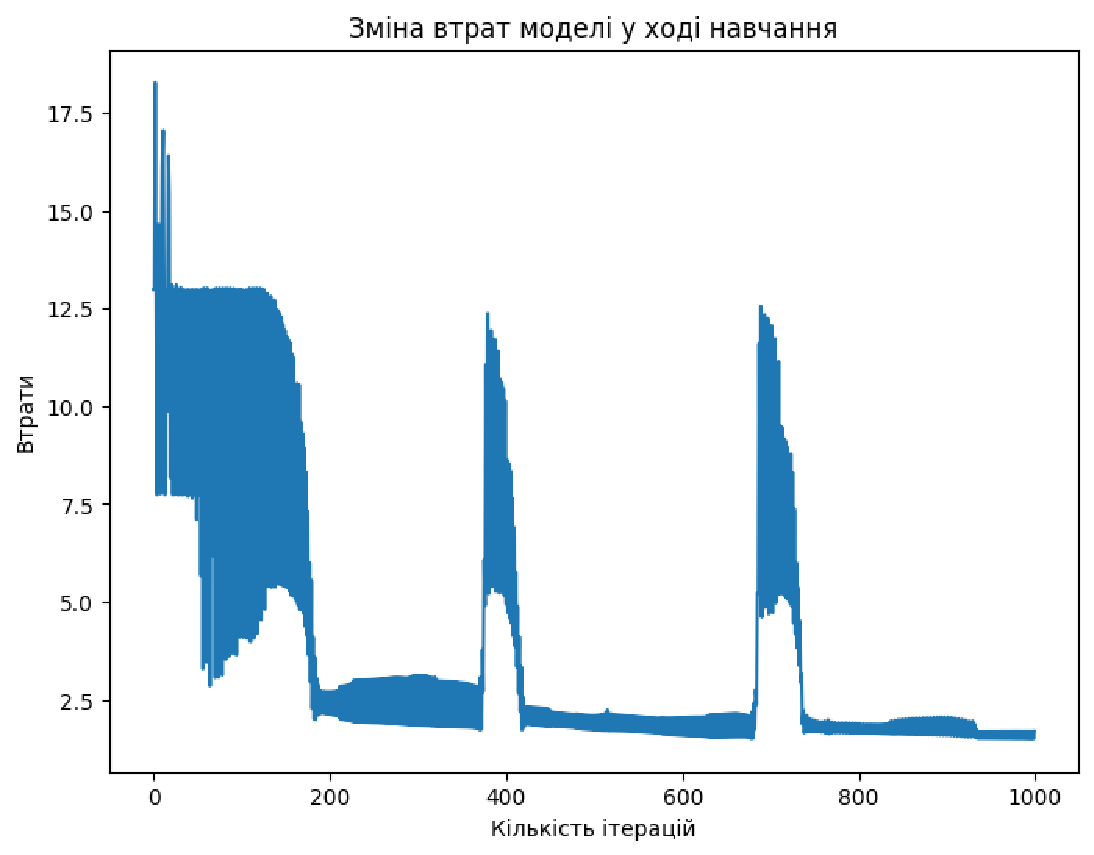
\includegraphics[scale=0.85]{1}
  \caption{Усереднена втрата моделі = 1.4424301845155454.}
  \label{im:1}
\end{figure}

Оскільки рисунок~\ref{im:1} показує перший варінт графіку, то відповідно немає з чим порівнювати. Для початку збільшимо кількість ітерацій в 10 разів щоб побачити певну закономірність

\begin{figure}[H]
  \center
  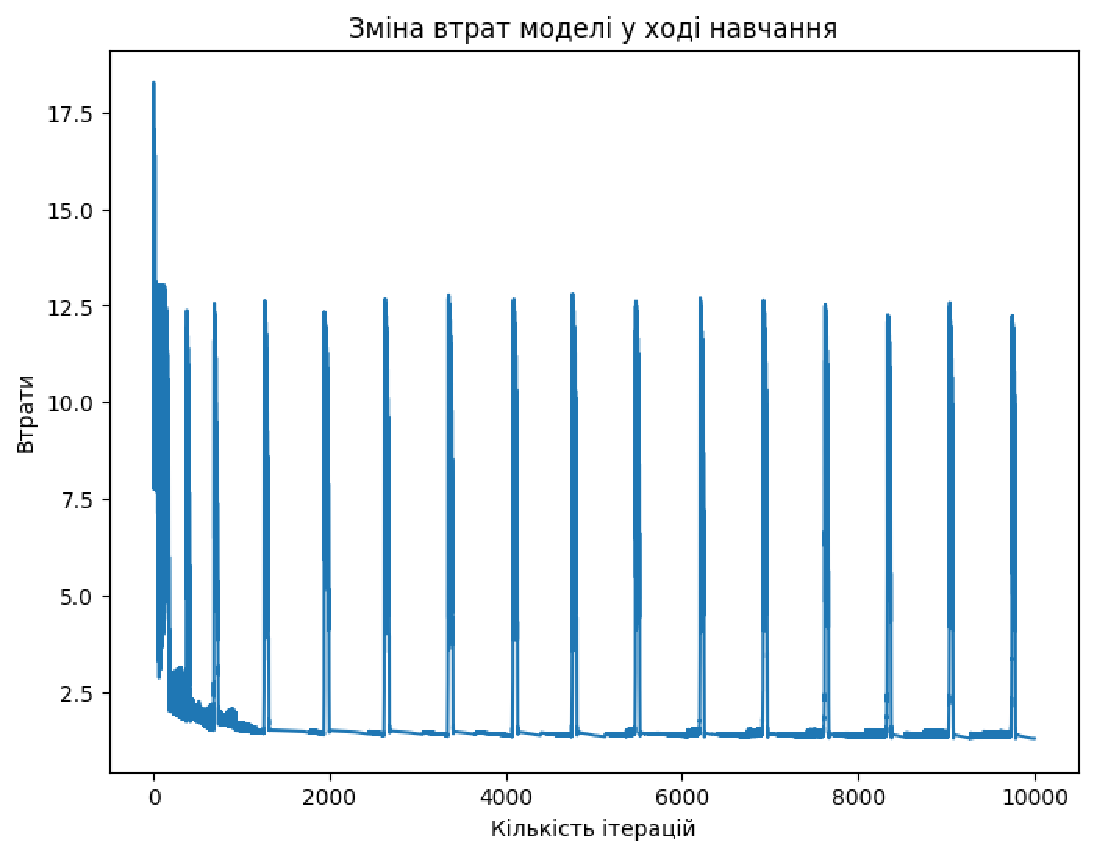
\includegraphics[scale=0.85]{2}
  \caption{Усереднена втрата моделі = 1.0749513733008609.}
  \label{im:2}
\end{figure}

Як ми бачимо на рисунку~\ref{im:2} після збільшення ітерацій - збільшилось і кількість стрибків втрат. Спробуємо зменшити кількість ітерацій

\begin{figure}[H]
  \center
  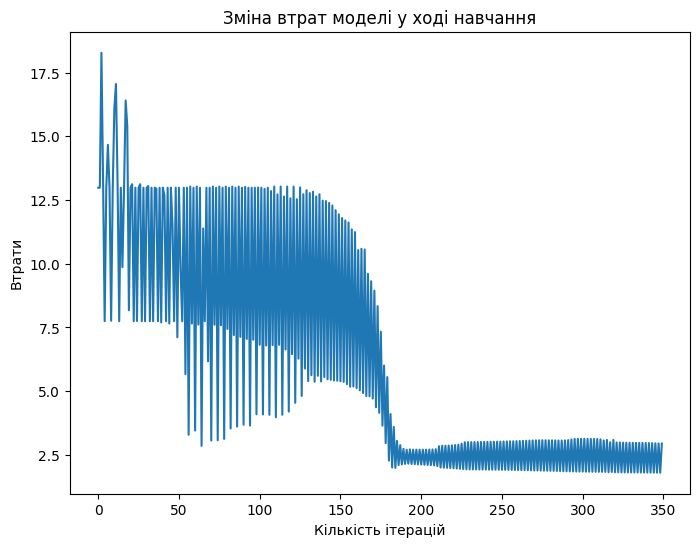
\includegraphics[scale=0.85]{3}
  \caption{Усереднена втрата моделі = 1.9528048260687907.}
  \label{im:3}
\end{figure}

Як ми бачимо на рисунку~\ref{im:3} графік стрибає, проте поступово підходить до мінімального значення втрат. Але все ж таки присутня ось цей стрибок у втратах та здається маються ознаки перетренування

\subsubsection{lr = 0.0001}

Зараз спробуємо подивитися на поведінку графіка при зменшенні швидкості навчання

\begin{figure}[H]
  \center
  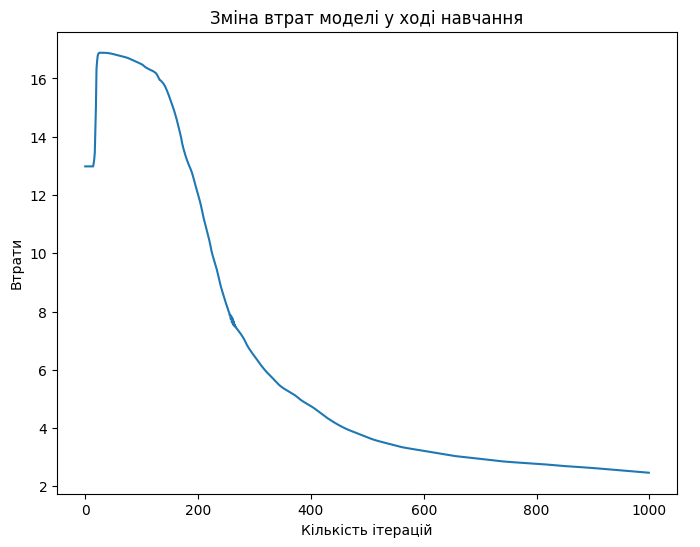
\includegraphics[scale=0.85]{4}
  \caption{Усереднена втрата моделі = 2.5209633875774364.}
  \label{im:4}
\end{figure}

Судячи з рисунку~\ref{im:4} бачимо що втрата хоча і більша, проте графік втрат стрибає менше. Спробуємо збільшити кількість ітерацій.

\begin{figure}[H]
  \center
  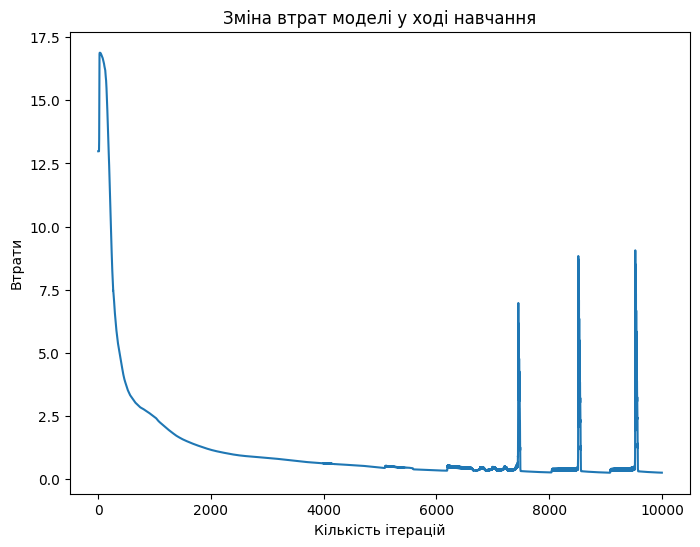
\includegraphics[scale=0.85]{5}
  \caption{Усереднена втрата моделі = 0.29179701311397743.}
  \label{im:5}
\end{figure}

Як бачимо на рисунку~\ref{im:5} ознаки перетренування з'являються тільки після 6000 ітерацій. Та втрата моделі мінімальна за всі спроби тестування. Спробуємо зменшити кількість ітерацій.

\begin{figure}[H]
  \center
  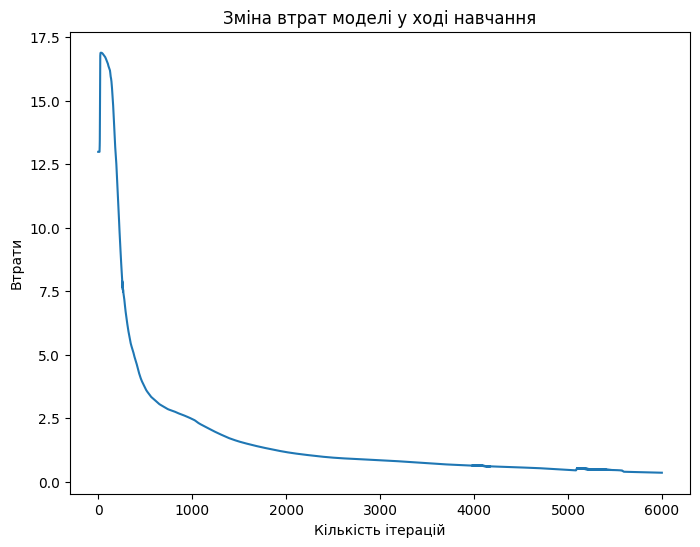
\includegraphics[scale=0.85]{6}
  \caption{Усереднена втрата моделі = 0.5231105268884676.}
  \label{im:6}
\end{figure}

Як ми бачимо на рисунку~\ref{im:6} графік виглядає достатньо гладким та відсутні ознаки перетренування

\subsubsection{lr = 0.01}

Зараз спробуємо збільшити швідкість навчання порівнянно зі стартовим значенням та проведемо відповідні спостереження.

\begin{figure}[H]
  \center
  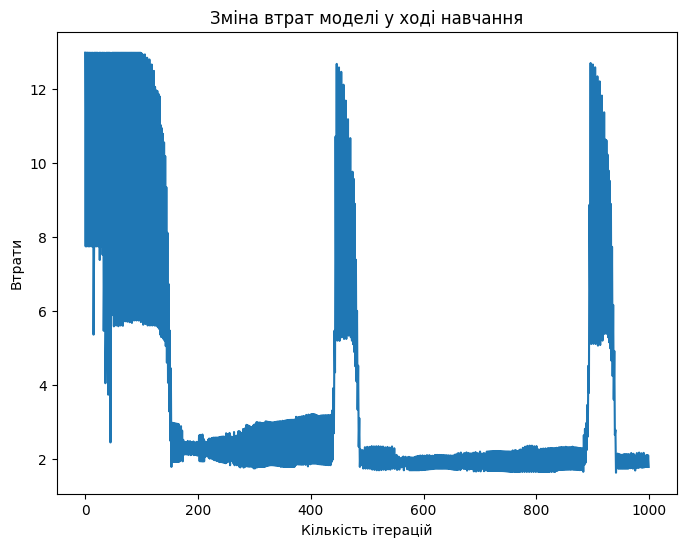
\includegraphics[scale=0.85]{7}
  \caption{Усереднена втрата моделі = 2.389146863129543.}
  \label{im:7}
\end{figure}

Як ми бачимо на рисунку~\ref{im:7} через збільшену швидкість навчання графік втрат також сильно стрибає, про що і кажуть жирні лінії.

\begin{figure}[H]
  \center
  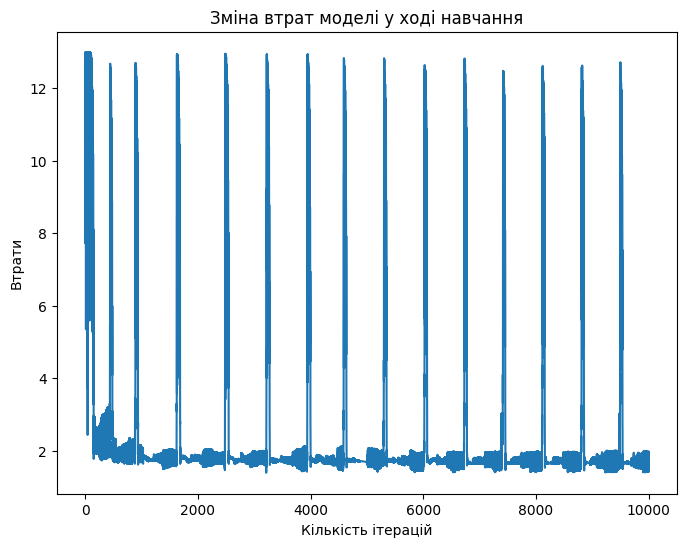
\includegraphics[scale=0.85]{8}
  \caption{Усереднена втрата моделі = 1.6360477068827715.}
  \label{im:8}
\end{figure}

При збільшенні ітерацій на рисунку~\ref{im:8} підтвеждується перетренування - що і очікувано.

\begin{figure}[H]
  \center
  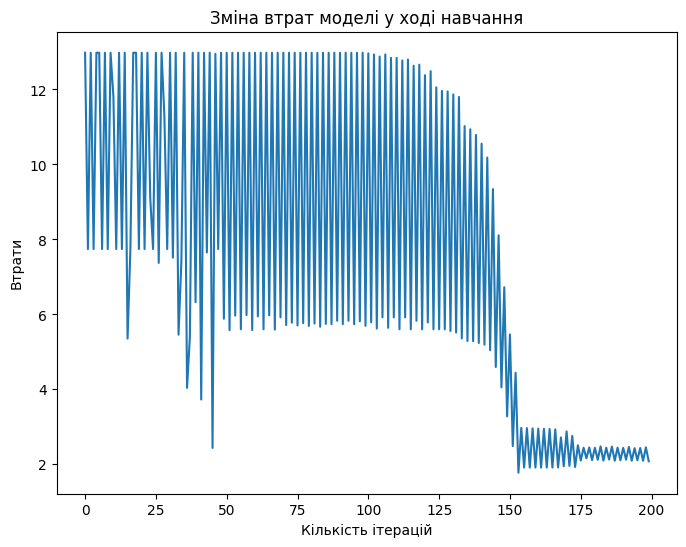
\includegraphics[scale=0.85]{9}
  \caption{Усереднена втрата моделі = 1.6360577568443848.}
  \label{im:9}
\end{figure}

При зменшенні ітерацій на рисунку~\ref{im:9} бачимо наскільки сильно стрибають втрати від ітерації до ітерації. А також бачимо що дуже погано сходиться

% \subsubsection{}

% Для представлення результатів використовуйте таблиці, графіки, рисунки. Приклад таблиці~\ref{tab:arithmetic}. Приклад рисунку~\ref{im:NN}.


% TODO таблиця в кінці після тестів
% #     lr        n_iters     accuracy
% 1     0.001     1000        1.4424301845155454
% 2     0.001     10000       1.0749513733008609
% 3     0.001     350         1.9528048260687907
% 4     0.0001    1000        2.5209633875774364
% 5     0.0001    10000       0.29179701311397743
% 6     0.0001    6000        0.5231105268884676
% 7     0.01      1000        2.389146863129543
% 8     0.01      10000       1.6360477068827715
% 9     0.01      200         1.6360577568443848

% \begin{table}[H]
%   \caption{Приклад таблиці.}
%   \label{tab:arithmetic}
%   \begin{center}
%     \begin{tabular}{ |>{\centering}p{5cm}|c|>{\centering}p{2.2cm}| }
%       \hline
%       \rowcolor{lightgray} \multicolumn{2}{|c|}{Ім'я оператора} & Синтаксис \tabularnewline
%       \hline
%       \multicolumn{2}{|c|}{Присвоєння}                          & a = b \tabularnewline
%       \hline
%       \multicolumn{2}{|c|}{Додавання}                           & a + b  \tabularnewline
%       \hline
%       \multicolumn{2}{|c|}{Віднімання}                          & a - b  \tabularnewline
%       \hline
%       \multicolumn{2}{|c|}{Унарний плюс}                        & +a   \tabularnewline
%       \hline
%       \multicolumn{2}{|c|}{Унарний мінус}                       & -a  \tabularnewline
%       \hline
%       \multicolumn{2}{|c|}{Множення}                            & a * b \tabularnewline
%       \hline
%       \multicolumn{2}{|c|}{Ділення}                             & a / b \tabularnewline
%       \hline
%       \multicolumn{2}{|c|}{Залишок від ділення}                 & a \% b \tabularnewline
%       \hline
%       \multirow{2}{*}{Інкремент}                                & префікс                   & ++a  \tabularnewline
%                                                                 & суфікс                    & a++  \tabularnewline
%       \hline
%       \multirow{2}{*}{Декремент}                                & префікс                   & - -a  \tabularnewline

%                                                                 & суфікс                    & a- -  \tabularnewline
%       \hline
%     \end{tabular}
%   \end{center}
% \end{table}

% \begin{figure}[!htb]
%   \center
%   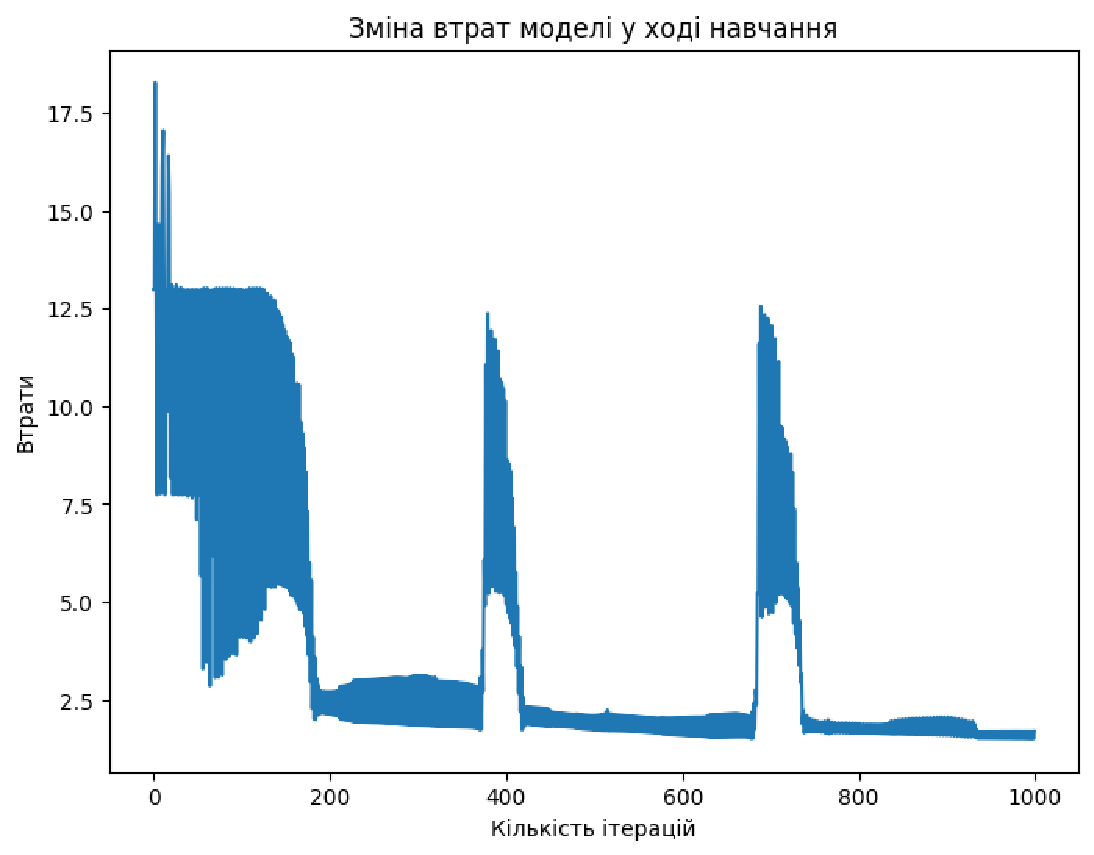
\includegraphics[scale=0.85]{1}
%   \caption{Приклад представлення нейронної мережі.}
%   \label{im:NN}
% \end{figure}

\subsection{Допомога}

Ну, по більшій частині задавав питання ChatGPT (якщо потрібно по буде по особистому запису можу дати посилання на відповідну сессію з питаннями) та трохи подивився вже існуючий аналіз цього ж датасету від HamnaKhalid~\cite{HamnaKhalidВС}, де використовується не тільки логістична регресія. Не використовував чужі матеріали (код / графіки / текст).


\subsection{Висновки}

Судячи с проведених тестів, можна сказати що най оптимальнішим буде вибір певного компромісу з повільності швидкості навчання та відповідній до неї кількості ітерацій, щоб модель не перенавчалась та ці значення - швидкість навчання ~0.0001 та кількість ітерацій ~6000. Проте варто зауважити що це саме такі результати для саме цієї моделі, данних та задачі.

\newpage
%%%%%%%%%%%%%%%%%% Література %%%%%%%%%%%%%%%%%%%%%%%%%%%%%%%%%%%%%%%%%%%%%%%
\clearpage
\bibliographystyle{IEEEtran}
\bibliography{ref}
\end{document}
